\section{What is ML?}
First some words about ML. Maybe from Lotz, first chapter?
Next we could use this graphic to visualize the topic.
\begin{figure}[hbtp]
	\centering
	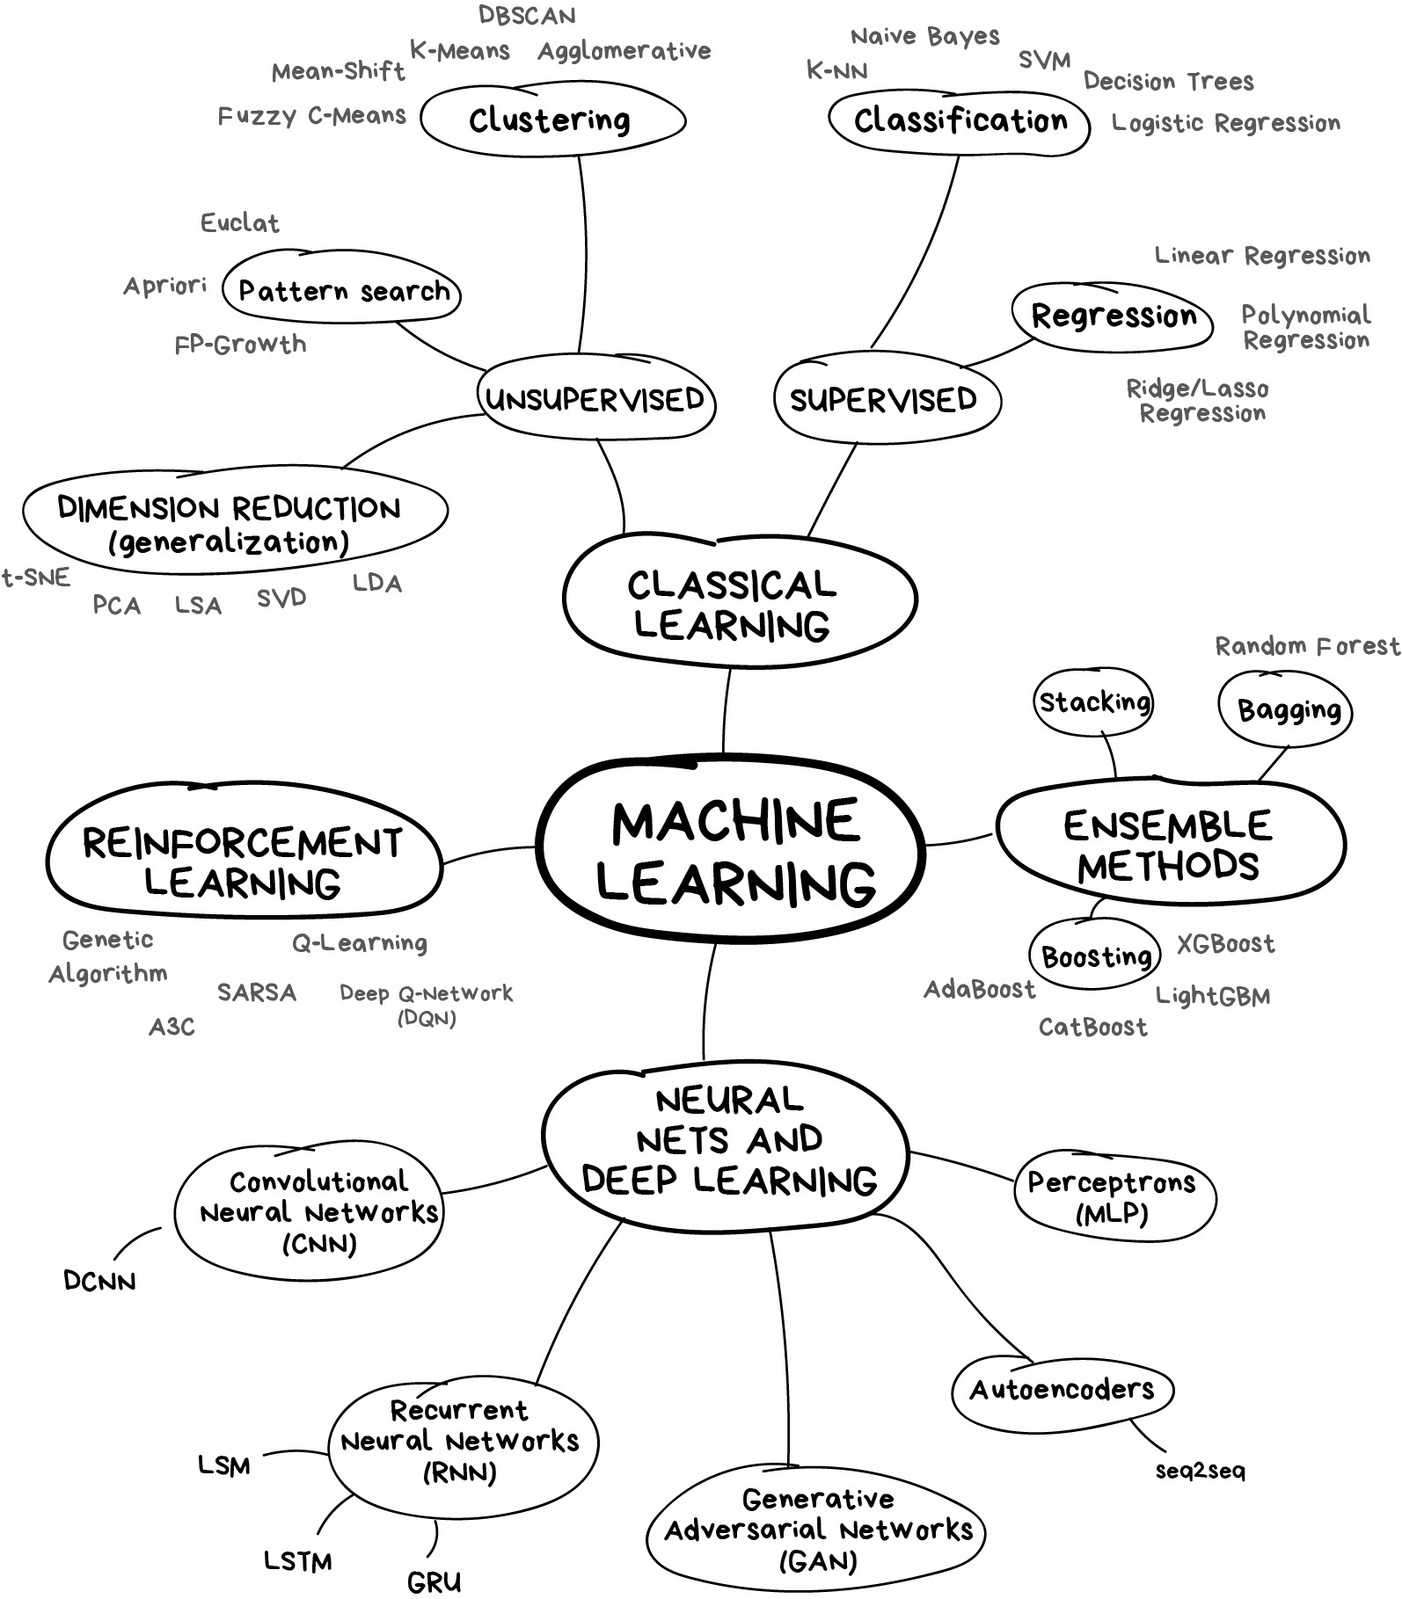
\includegraphics[width=1\textwidth]{ML}
	\caption{ML-Overview}
	% \vspace{-20pt}
	\label{fig:Datensatz - unbearbeitet}
\end{figure}

Finally i would suggest to finish with a Table.

I would structure it like:
Algorithm, Main Idea(in like 3-5 sentences), possible application(image processing, clustering, etc.) advantages, disadvantages

%%%%%%%%%%%%%%%%%%%%%%%%%%%%%%%%%%%%%%%%%%%%%%%%%%%%%%%%%

\subsection{Basis ML 1(maybe Data)}
We could speak a lil bit more about data in this topic?




%%%%%%%%%%%%%%%%%%%%%%%%%%%%%%%%%%%%%%%%%%%%%%%%%%%%%%%%%

\subsection{Basis ML 2}
TBA





\newpage